\subsubsection{UC3 - Login}
\begin{itemize}
\item \textbf{Attori primari}: utente non autenticato;
\item \textbf{Descrizione}: l'utente, inserendo le proprie credenziali, viene autenticato alla piattaforma;
\item \textbf{Scenario Principale}: l'utente non ancora autenticato inizia la procedura di login tramite l'apposito pulsante, inserisce le proprie credenziali \textbf{[UC3.1]} e richiede il login \textbf{[UC3.2]};
\item \textbf{Estensioni}:
\begin{itemize}
	\item \textbf{UC4}: se le credenziali inserite non vengono riconosciute dall'Identity Manager, viene visualizzato un messaggio che informa l'utente dell'errore.
\end{itemize}
\item \textbf{Precondizione}: l'utente prova ad autenticarsi alla piattaforma;
\item \textbf{Postcondizione}: l'utente viene autenticato come cliente o come venditore.
\end{itemize}

\begin{figure}[H]
\centering
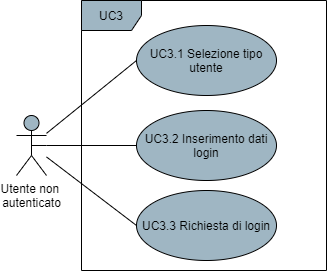
\includegraphics[scale=0.6]{res/UseCase/Immagini/LoginSottocasi}
\caption{Diagramma UML\ped{G} per UC3 - Login}
\end{figure}

\subsubsection{UC3.1 - Inserimento dati login}
\begin{itemize}
\item \textbf{Attori primari}: utente non autenticato;
\item \textbf{Descrizione}: l'utente compila il form per il login;
\item \textbf{Scenario Principale}: l'utente inserisce nel form apposito i dati necessari al login;
\item \textbf{Precondizione}: il form di inserimento dati per il login è disponibile;
\item \textbf{Postcondizione}: i dati necessari al login sono stati compilati.
\end{itemize}

\begin{figure}[H]
\centering
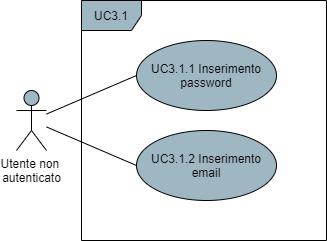
\includegraphics[scale=0.6]{res/UseCase/Immagini/InserimentoDatiLogin}
\caption{Diagramma UML\ped{G} per UC3.1 - Inserimento dati login}
\end{figure}

\subsubsection{UC3.1.1 - Inserimento password}
\begin{itemize}
\item \textbf{Attori primari}: utente non autenticato;
\item \textbf{Descrizione}: l'utente deve compilare il campo "Password" per procedere al login;
\item \textbf{Scenario Principale}: l'utente inserisce la sua password nell'apposito campo;
\item \textbf{Precondizione}: il campo "Password" risulta vuoto;
\item \textbf{Postcondizione}: il campo "Password" è stato compilato.
\end{itemize}

\subsubsection{UC3.1.2 - Inserimento email}
\begin{itemize}
\item \textbf{Attori primari}: utente non autenticato;
\item \textbf{Descrizione}: l'utente deve compilare il campo "Email" per procedere al login;
\item \textbf{Scenario Principale}: l'utente inserisce il suo indirizzo email nell'apposito campo;
\item \textbf{Precondizione}: il campo "Email" risulta vuoto;
\item \textbf{Postcondizione}: il campo "Email" è stato compilato.
\end{itemize}

\subsubsection{UC3.2 - Richiesta di login}
\begin{itemize}
\item \textbf{Attori primari}: utente non autenticato;
\item \textbf{Descrizione}: l'utente richiede l'autenticazione con i dati inseriti;
\item \textbf{Scenario Principale}: l'utente preme il tasto di login e manda la richiesta al sistema con i dati presenti nel form;
\item \textbf{Precondizione}: l'utente prova ad autenticarsi alla piattaforma;
\item \textbf{Postcondizione}: la richiesta di login è stata mandata al sistema.
\end{itemize} 

\subsubsection{UC4 - Visualizzazione errore dati login errati}
\begin{itemize}
\item \textbf{Attori primari}: utente non autenticato;
\item \textbf{Descrizione}: l'utente visualizza un messaggio di errore che lo informa che i dati da lui inseriti durante il login non sono riconosciuti dall'Identity Manager;
\item \textbf{Scenario Principale}: l'utente tenta di effettuare il login usando credenziali non presenti nel sistema;
\item \textbf{Precondizione}: l'utente prova ad autenticarsi alla piattaforma;
\item \textbf{Postcondizione}: viene visualizzato un messaggio che informa l'utente dell'errore di riconoscimento delle credenziali.
\end{itemize}